%!TEX root = ../thesis.tex

\thispagestyle{myheadings}

\graphicspath{{Body/Figures/Wa/Datasets/60h/BunchNum/}{Body/Figures/Wa/Datasets/HighKick/BunchNum/}{Body/Figures/Wa/Datasets/9d/BunchNum/}{Body/Figures/Wa/Datasets/Endgame/BunchNum/}{Body/Figures/Wa/Datasets/60h/SingleIteration/FitStartScans/}{Body/Figures/Wa/Datasets/HighKick/SingleIteration/FitStartScans/}{Body/Figures/Wa/Datasets/9d/SingleIteration/FitStartScans/}{Body/Figures/Wa/Datasets/Endgame/SingleIteration/FitStartScans/}{Body/Figures/Wa/Datasets/60h/SingleIteration/FitEndScans/}{Body/Figures/Wa/Datasets/HighKick/SingleIteration/FitEndScans/}{Body/Figures/Wa/Datasets/9d/SingleIteration/FitEndScans/}{Body/Figures/Wa/Datasets/Endgame/SingleIteration/FitEndScans/}{Body/Figures/Wa/Datasets/60h/EnergyThreshold/}{Body/Figures/Wa/Datasets/HighKick/EnergyThreshold/}{Body/Figures/Wa/Datasets/9d/EnergyThreshold/}{Body/Figures/Wa/Datasets/Endgame/EnergyThreshold/}{Body/Figures/Wa/Datasets/60h/RandSeeds/}{Body/Figures/Wa/Datasets/HighKick/RandSeeds/}{Body/Figures/Wa/Datasets/9d/RandSeeds/}{Body/Figures/Wa/Datasets/Endgame/RandSeeds/}{Body/Figures/Wa/Datasets/60h/SingleIteration/CaloFits/}{Body/Figures/Wa/Datasets/HighKick/SingleIteration/CaloFits/}{Body/Figures/Wa/Datasets/9d/SingleIteration/CaloFits/}{Body/Figures/Wa/Datasets/Endgame/SingleIteration/CaloFits/}{Body/Figures/Wa/Datasets/60h/SingleIteration/SingleFits/}{Body/Figures/Wa/Datasets/HighKick/SingleIteration/SingleFits/}{Body/Figures/Wa/Datasets/9d/SingleIteration/SingleFits/}{Body/Figures/Wa/Datasets/Endgame/SingleIteration/SingleFits/}}




\section{Fit results}

Fit results are blah from a single random seed ... 





Ratio Method fits including the CBO terms typically converge with lifetimes with large errors compared to T-Method fits, due to the reduction in sensitivity in the Ratio Method. In the HighKick dataset specifically, the CBO lifetime which is smaller than the other datasets does not like to converge nicely in the ratio fits, and is therefore fixed to that from a T-Method fit.


I should show an FFT of the ratio fit residuals 



-put here paramter values and all that for single seed fits to the individual datasets
-modulo plots
-maybe correlation matrix plots - or maybe those go into an appendix
-include FFT plots and pull plots 
-perhaps include or reference the average value of R

-only show 60h residuals and fft?



\begin{figure}[]
    \centering
    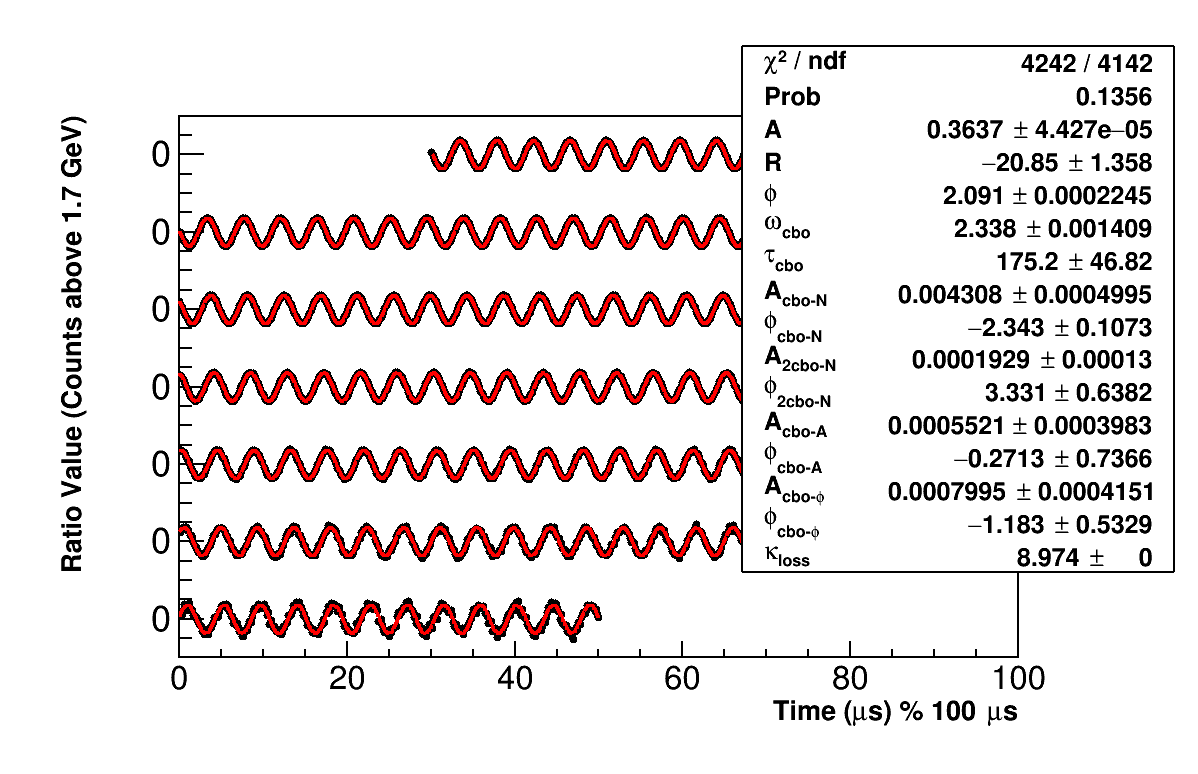
\includegraphics[width=\textwidth]{fullRatio_moduloPlot_60h}
    \caption[]{Data from some dataset.}
    \label{fig:}
\end{figure}


\begin{figure}[]
    \centering
    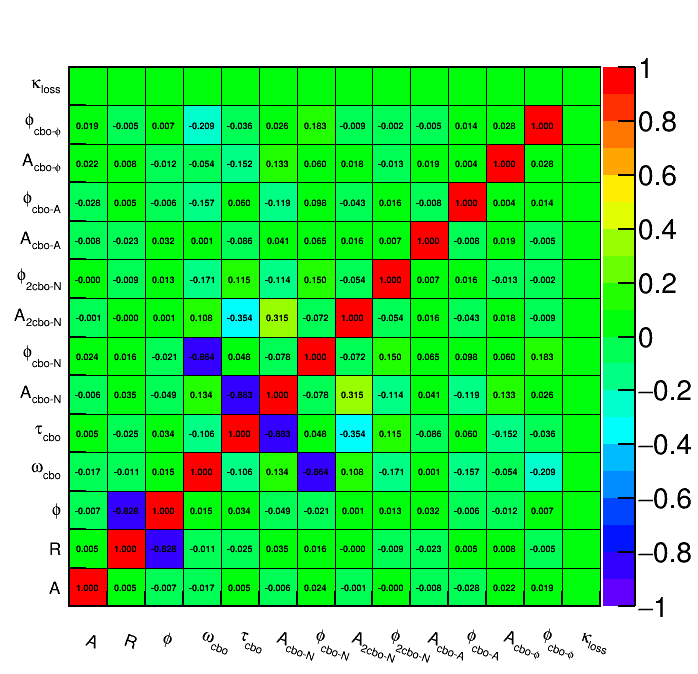
\includegraphics[width=\textwidth]{CorrelationMatrixFullRatioFit_60h}
    \caption[]{Data from some dataset.}
    \label{fig:}
\end{figure}


\begin{landscape}
\begin{table}[]
\setlength\tabcolsep{5pt}
\footnotesize
\begin{tabular*}{\linewidth}{@{\extracolsep{\fill}}lLBLLLLLLLLLLLL}
  \toprule
            & \thead{$A$} & \thead{$R$} & \thead{$\phi$} & \thead{$\omega_{cbo}$} & \thead{$\tau_{cbo}$} & \thead{$A_{cbo-N}$} & \thead{$\phi_{cbo-N}$} & \thead{$A_{2cbo-N}$} & \thead{$\phi_{2cbo-N}$} & \thead{$A_{cbo-A}$} & \thead{$\phi_{cbo-A}$} & \thead{$A_{cbo-\phi}$} & \thead{$\phi_{cbo-\phi}$} & \thead{$\kappa_{loss}$} \\
  \midrule
$A$                & 1.000 & 0.005 & -0.007 & -0.017 & 0.005 & -0.006 & 0.024 & -0.001 & -0.000 & -0.008 & -0.028 & 0.022 & 0.019 & 0.000  \\
$R$                & 0.005 & 1.000 & -0.828 & -0.011 & -0.025 & 0.035 & 0.016 & -0.000 & -0.009 & -0.023 & 0.005 & 0.008 & -0.005 & 0.000  \\
$\phi$             & -0.007 & -0.828 & 1.000 & 0.015 & 0.034 & -0.049 & -0.021 & 0.001 & 0.013 & 0.032 & -0.006 & -0.012 & 0.007 & 0.000  \\
$\omega_{cbo}$     & -0.017 & -0.011 & 0.015 & 1.000 & -0.106 & 0.134 & -0.864 & 0.108 & -0.171 & 0.001 & -0.157 & -0.054 & -0.209 & 0.000  \\
$\tau_{cbo}$       & 0.005 & -0.025 & 0.034 & -0.106 & 1.000 & -0.883 & 0.048 & -0.354 & 0.115 & -0.086 & 0.060 & -0.152 & -0.036 & 0.000  \\
$A_{cbo-N}$        & -0.006 & 0.035 & -0.049 & 0.134 & -0.883 & 1.000 & -0.078 & 0.315 & -0.114 & 0.041 & -0.119 & 0.133 & 0.026 & 0.000  \\
$\phi_{cbo-N}$     & 0.024 & 0.016 & -0.021 & -0.864 & 0.048 & -0.078 & 1.000 & -0.072 & 0.150 & 0.065 & 0.098 & 0.060 & 0.183 & 0.000  \\
$A_{2cbo-N}$       & -0.001 & -0.000 & 0.001 & 0.108 & -0.354 & 0.315 & -0.072 & 1.000 & -0.054 & 0.016 & -0.043 & 0.018 & -0.009 & 0.000  \\
$\phi_{2cbo-N}$    & -0.000 & -0.009 & 0.013 & -0.171 & 0.115 & -0.114 & 0.150 & -0.054 & 1.000 & 0.007 & 0.016 & -0.013 & -0.002 & 0.000  \\
$A_{cbo-A}$        & -0.008 & -0.023 & 0.032 & 0.001 & -0.086 & 0.041 & 0.065 & 0.016 & 0.007 & 1.000 & -0.008 & 0.019 & -0.005 & 0.000  \\
$\phi_{cbo-A}$     & -0.028 & 0.005 & -0.006 & -0.157 & 0.060 & -0.119 & 0.098 & -0.043 & 0.016 & -0.008 & 1.000 & 0.004 & 0.014 & 0.000  \\
$A_{cbo-\phi}$     & 0.022 & 0.008 & -0.012 & -0.054 & -0.152 & 0.133 & 0.060 & 0.018 & -0.013 & 0.019 & 0.004 & 1.000 & 0.028 & 0.000  \\
$\phi_{cbo-\phi}$  & 0.019 & -0.005 & 0.007 & -0.209 & -0.036 & 0.026 & 0.183 & -0.009 & -0.002 & -0.005 & 0.014 & 0.028 & 1.000 & 0.000  \\
$\kappa_{loss}$    & 0.000 & 0.000 & 0.000 & 0.000 & 0.000 & 0.000 & 0.000 & 0.000 & 0.000 & 0.000 & 0.000 & 0.000 & 0.000 & 0.000  \\
  \bottomrule
\end{tabular*}
\caption[]{60h Correlation matrix for the full ratio fit. The only significant correlation to R is the \gmtwo phase.}
\label{Tab:CorrMat}
\end{table}
\end{landscape}


    \begin{figure}[h]
    \centering
        \begin{subfigure}[]{0.45\textwidth}
            \centering
            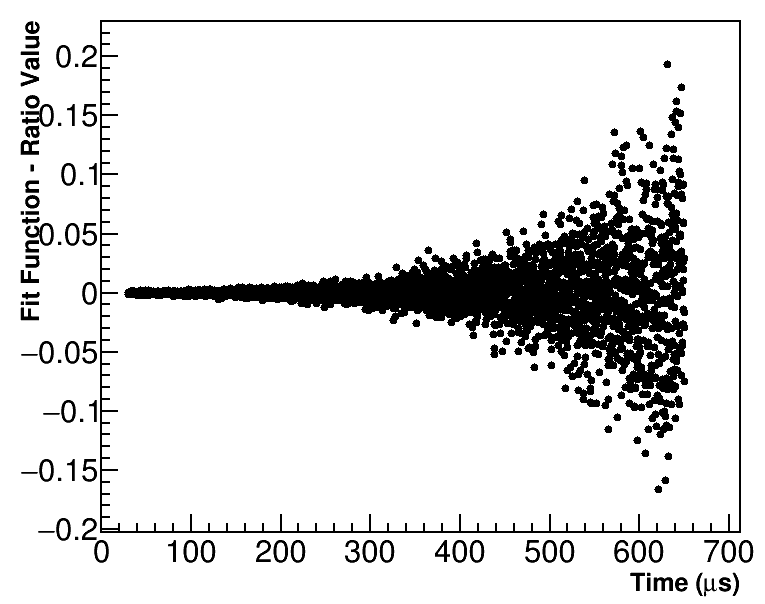
\includegraphics[width=\textwidth]{fitResidual_60h}
            \caption{Fit residuals.}
        \end{subfigure}
        \begin{subfigure}[]{0.45\textwidth}
            \centering
            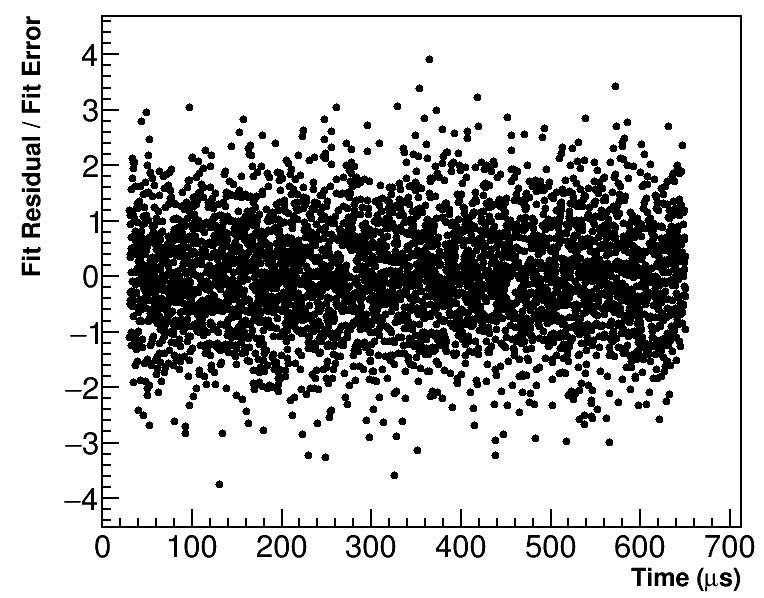
\includegraphics[width=\textwidth]{fitPull_60h}
            \caption{Fit pulls.}
        \end{subfigure}% %you need this % here to add spacing between subfigures
        \vspace{4mm}
        \begin{subfigure}[]{0.7\textwidth}
            \centering
            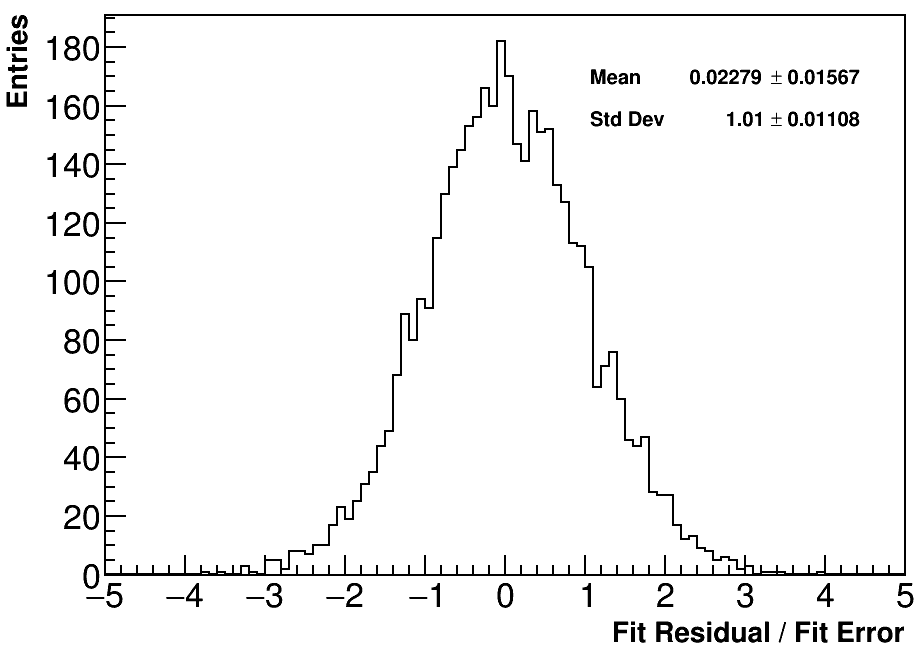
\includegraphics[width=\textwidth]{fitPull_projected_60h}
            \caption{Fit pulls projected onto the y axis. Note the Gaussian shape centered around 0 with unit width.}
        \end{subfigure}
    \caption[fitResidual]{Residuals and pulls for the full ratio fit. \textbf{fix up}}
    \label{fig:fitResidual}
    \end{figure}


\begin{figure}[]
    \centering
    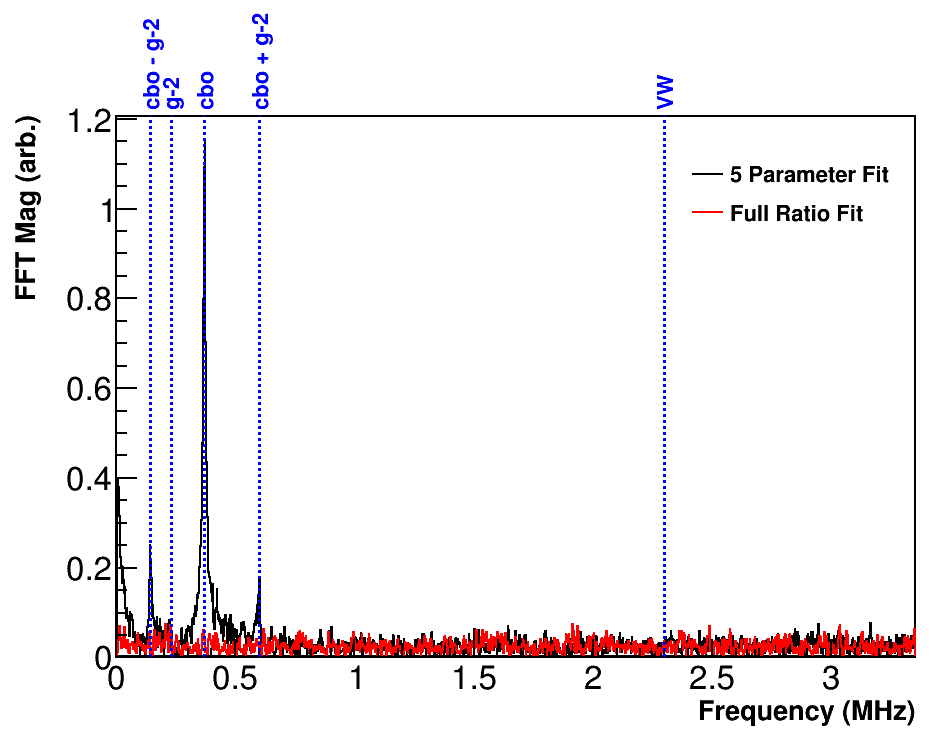
\includegraphics[width=\textwidth]{FFTComparison_FullRatio_60h}
    \caption[]{Data from some dataset.}
    \label{fig:}
\end{figure}



\begin{figure}[]
    \centering
    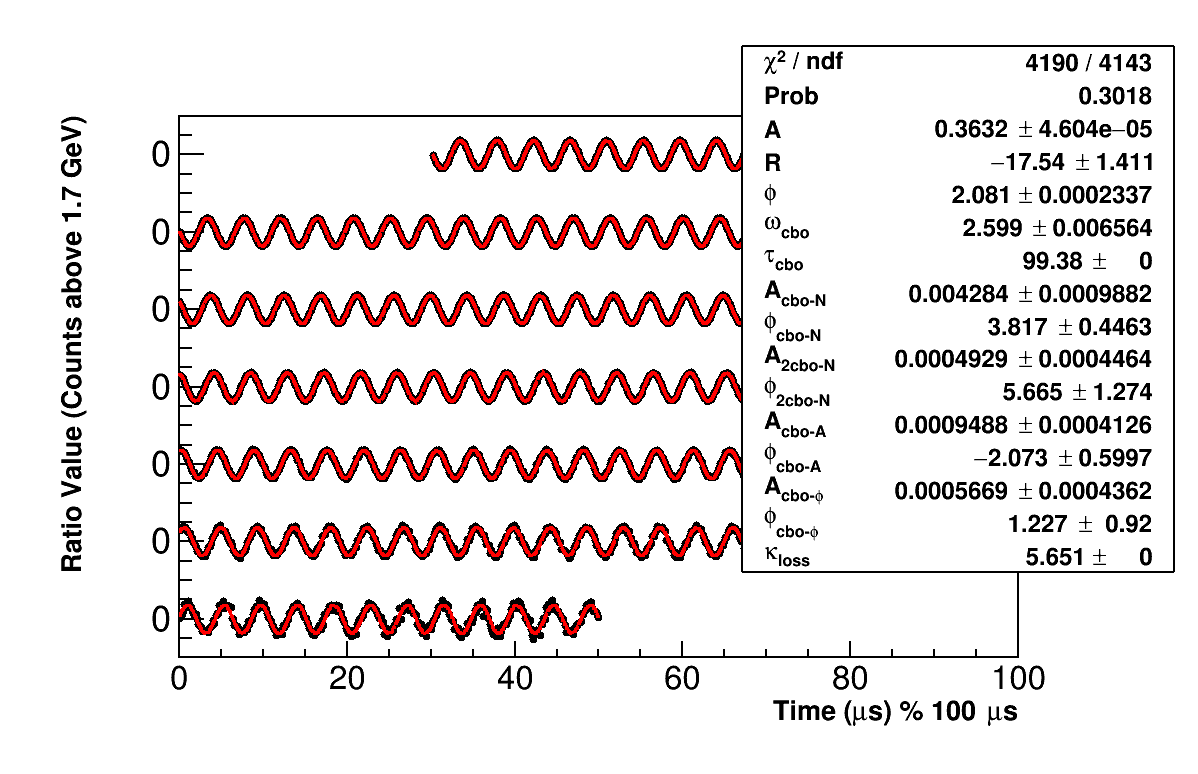
\includegraphics[width=\textwidth]{fullRatio_moduloPlot_HighKick}
    \caption[]{Data from some dataset.}
    \label{fig:}
\end{figure}

\begin{figure}[]
    \centering
    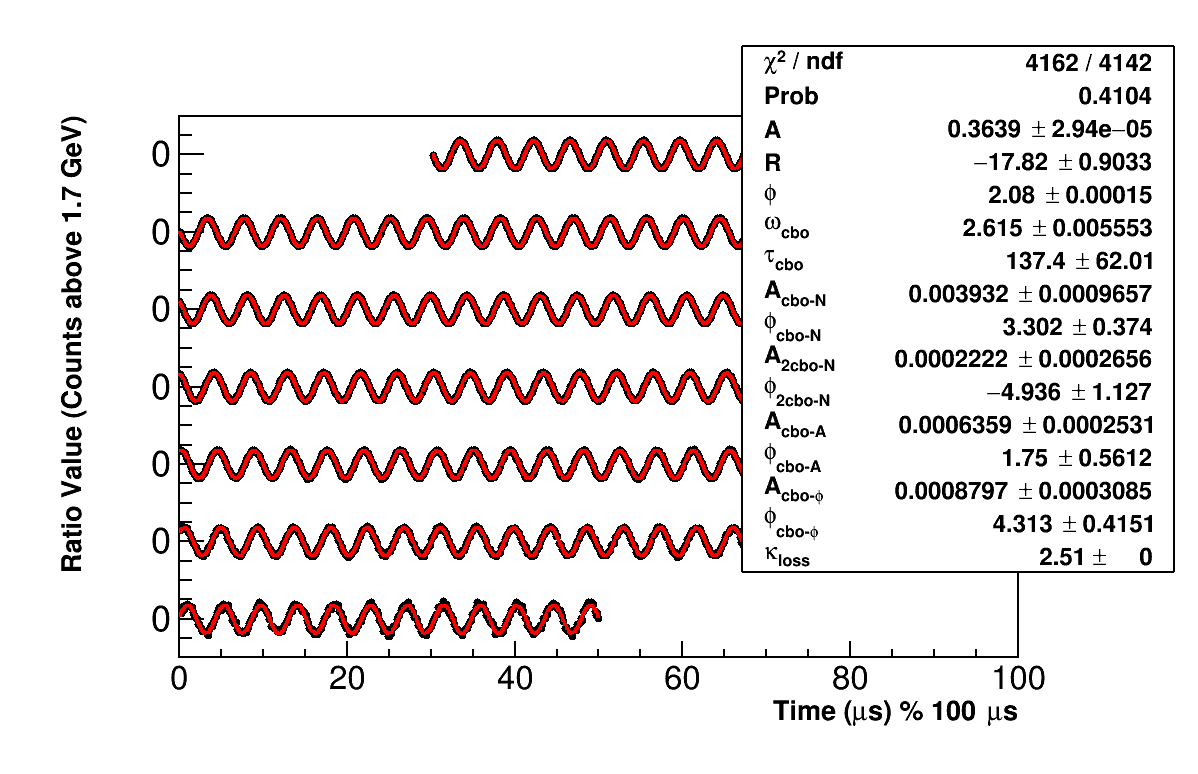
\includegraphics[width=\textwidth]{fullRatio_moduloPlot_9d}
    \caption[]{Data from some dataset.}
    \label{fig:}
\end{figure}

\begin{figure}[]
    \centering
    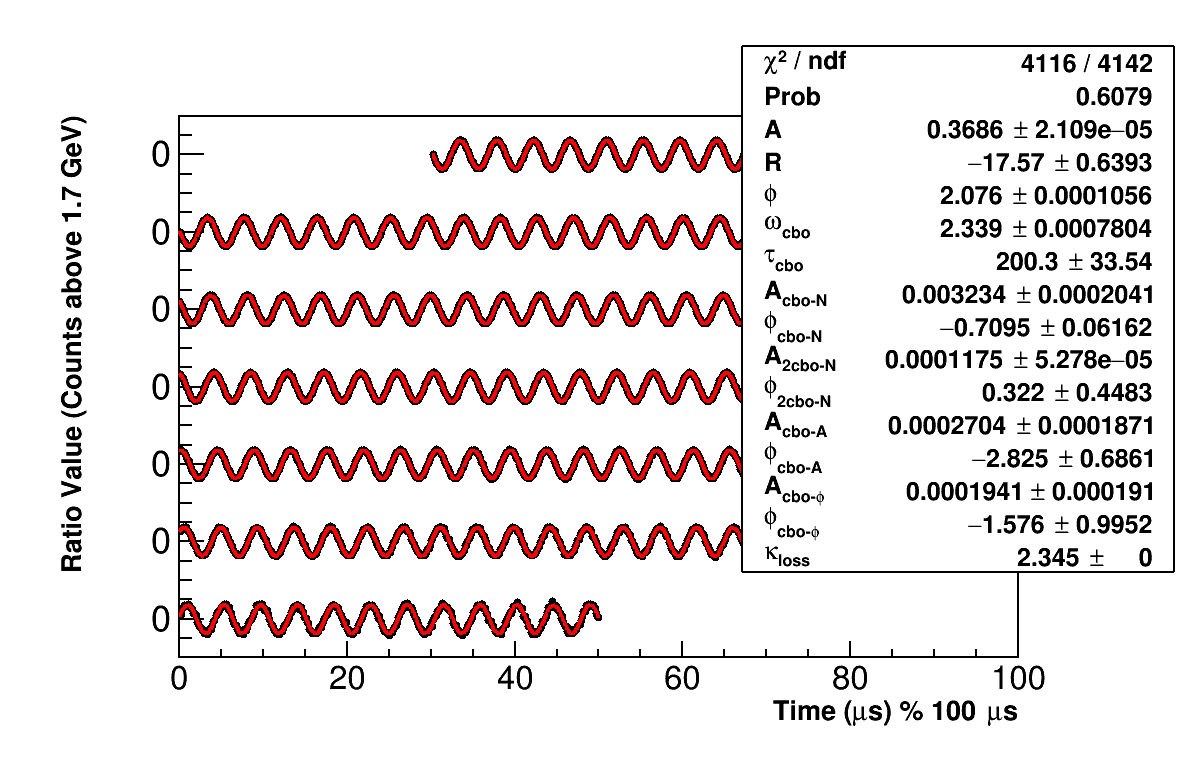
\includegraphics[width=\textwidth]{fullRatio_moduloPlot_Endgame}
    \caption[]{Data from some dataset.}
    \label{fig:}
\end{figure}

\begin{landscape}
\begin{table}[]
\setlength\tabcolsep{5pt}
\footnotesize
\begin{tabular*}{\linewidth}{@{\extracolsep{\fill}}lLBLLLLLLLLLLLL}
  \toprule
            & \thead{$A$} & \thead{$R$} & \thead{$\phi$} & \thead{$\omega_{cbo}$} & \thead{$\tau_{cbo}$} & \thead{$A_{cbo-N}$} & \thead{$\phi_{cbo-N}$} & \thead{$A_{2cbo-N}$} & \thead{$\phi_{2cbo-N}$} & \thead{$A_{cbo-A}$} & \thead{$\phi_{cbo-A}$} & \thead{$A_{cbo-\phi}$} & \thead{$\phi_{cbo-\phi}$} & \thead{$\kappa_{loss}$} \\
  \midrule
$A$                & 1.000 & 0.005 & -0.007 & 0.031 & 0.000 & 0.022 & -0.024 & 0.008 & -0.022 & 0.006 & -0.066 & -0.059 & -0.018 & 0.000  \\
$R$                & 0.005 & 1.000 & -0.828 & 0.012 & 0.000 & 0.022 & -0.022 & 0.007 & -0.017 & -0.053 & -0.012 & 0.003 & 0.021 & 0.000  \\
$\phi$             & -0.007 & -0.828 & 1.000 & -0.017 & 0.000 & -0.031 & 0.031 & -0.010 & 0.024 & 0.073 & 0.019 & -0.002 & -0.028 & 0.000  \\
$\omega_{cbo}$     & 0.031 & 0.012 & -0.017 & 1.000 & 0.000 & 0.233 & -0.861 & 0.108 & -0.701 & -0.041 & -0.690 & -0.236 & -0.577 & 0.000  \\
$\tau_{cbo}$       & 0.000 & 0.000 & 0.000 & 0.000 & 0.000 & 0.000 & 0.000 & 0.000 & 0.000 & 0.000 & 0.000 & 0.000 & 0.000 & 0.000  \\
$A_{cbo-N}$        & 0.022 & 0.022 & -0.031 & 0.233 & 0.000 & 1.000 & -0.203 & 0.020 & -0.150 & 0.045 & -0.184 & -0.068 & -0.127 & 0.000  \\
$\phi_{cbo-N}$     & -0.024 & -0.022 & 0.031 & -0.861 & 0.000 & -0.203 & 1.000 & -0.101 & 0.608 & 0.050 & 0.617 & 0.205 & 0.500 & 0.000  \\
$A_{2cbo-N}$       & 0.008 & 0.007 & -0.010 & 0.108 & 0.000 & 0.020 & -0.101 & 1.000 & -0.073 & -0.029 & -0.074 & -0.041 & -0.087 & 0.000  \\
$\phi_{2cbo-N}$    & -0.022 & -0.017 & 0.024 & -0.701 & 0.000 & -0.150 & 0.608 & -0.073 & 1.000 & 0.030 & 0.473 & 0.198 & 0.402 & 0.000  \\
$A_{cbo-A}$        & 0.006 & -0.053 & 0.073 & -0.041 & 0.000 & 0.045 & 0.050 & -0.029 & 0.030 & 1.000 & 0.025 & 0.013 & 0.020 & 0.000  \\
$\phi_{cbo-A}$     & -0.066 & -0.012 & 0.019 & -0.690 & 0.000 & -0.184 & 0.617 & -0.074 & 0.473 & 0.025 & 1.000 & 0.166 & 0.409 & 0.000  \\
$A_{cbo-\phi}$     & -0.059 & 0.003 & -0.002 & -0.236 & 0.000 & -0.068 & 0.205 & -0.041 & 0.198 & 0.013 & 0.166 & 1.000 & 0.148 & 0.000  \\
$\phi_{cbo-\phi}$  & -0.018 & 0.021 & -0.028 & -0.577 & 0.000 & -0.127 & 0.500 & -0.087 & 0.402 & 0.020 & 0.409 & 0.148 & 1.000 & 0.000  \\
$\kappa_{loss}$    & 0.000 & 0.000 & 0.000 & 0.000 & 0.000 & 0.000 & 0.000 & 0.000 & 0.000 & 0.000 & 0.000 & 0.000 & 0.000 & 0.000  \\
  \bottomrule
\end{tabular*}
\caption[]{highkick Correlation matrix for the full ratio fit. The only significant correlation to R is the \gmtwo phase.}
\label{Tab:CorrMat}
\end{table}
\end{landscape}

\begin{landscape}
\begin{table}[]
\setlength\tabcolsep{5pt}
\footnotesize
\begin{tabular*}{\linewidth}{@{\extracolsep{\fill}}lLBLLLLLLLLLLLL}
  \toprule
            & \thead{$A$} & \thead{$R$} & \thead{$\phi$} & \thead{$\omega_{cbo}$} & \thead{$\tau_{cbo}$} & \thead{$A_{cbo-N}$} & \thead{$\phi_{cbo-N}$} & \thead{$A_{2cbo-N}$} & \thead{$\phi_{2cbo-N}$} & \thead{$A_{cbo-A}$} & \thead{$\phi_{cbo-A}$} & \thead{$A_{cbo-\phi}$} & \thead{$\phi_{cbo-\phi}$} & \thead{$\kappa_{loss}$} \\
  \midrule
$A$                & 1.000 & 0.006 & -0.008 & 0.007 & -0.034 & 0.037 & -0.002 & 0.009 & 0.002 & 0.063 & 0.004 & 0.053 & -0.022 & 0.000  \\
$R$                & 0.006 & 1.000 & -0.829 & 0.084 & -0.001 & 0.018 & -0.085 & -0.011 & -0.008 & 0.043 & -0.096 & -0.024 & -0.082 & 0.000  \\
$\phi$             & -0.008 & -0.829 & 1.000 & -0.116 & 0.001 & -0.026 & 0.118 & 0.015 & 0.011 & -0.061 & 0.132 & 0.031 & 0.114 & 0.000  \\
$\omega_{cbo}$     & 0.007 & 0.084 & -0.116 & 1.000 & 0.074 & 0.036 & -0.912 & -0.123 & -0.240 & 0.282 & -0.781 & -0.138 & -0.788 & 0.000  \\
$\tau_{cbo}$       & -0.034 & -0.001 & 0.001 & 0.074 & 1.000 & -0.788 & -0.143 & -0.413 & -0.104 & -0.398 & 0.056 & -0.671 & -0.086 & 0.000  \\
$A_{cbo-N}$        & 0.037 & 0.018 & -0.026 & 0.036 & -0.788 & 1.000 & 0.027 & 0.319 & 0.049 & 0.347 & -0.099 & 0.523 & -0.012 & 0.000  \\
$\phi_{cbo-N}$     & -0.002 & -0.085 & 0.118 & -0.912 & -0.143 & 0.027 & 1.000 & 0.147 & 0.222 & -0.247 & 0.705 & 0.174 & 0.721 & 0.000  \\
$A_{2cbo-N}$       & 0.009 & -0.011 & 0.015 & -0.123 & -0.413 & 0.319 & 0.147 & 1.000 & 0.068 & 0.130 & 0.060 & 0.271 & 0.099 & 0.000  \\
$\phi_{2cbo-N}$    & 0.002 & -0.008 & 0.011 & -0.240 & -0.104 & 0.049 & 0.222 & 0.068 & 1.000 & -0.044 & 0.173 & 0.113 & 0.178 & 0.000  \\
$A_{cbo-A}$        & 0.063 & 0.043 & -0.061 & 0.282 & -0.398 & 0.347 & -0.247 & 0.130 & -0.044 & 1.000 & -0.268 & 0.247 & -0.206 & 0.000  \\
$\phi_{cbo-A}$     & 0.004 & -0.096 & 0.132 & -0.781 & 0.056 & -0.099 & 0.705 & 0.060 & 0.173 & -0.268 & 1.000 & 0.033 & 0.616 & 0.000  \\
$A_{cbo-\phi}$     & 0.053 & -0.024 & 0.031 & -0.138 & -0.671 & 0.523 & 0.174 & 0.271 & 0.113 & 0.247 & 0.033 & 1.000 & 0.131 & 0.000  \\
$\phi_{cbo-\phi}$  & -0.022 & -0.082 & 0.114 & -0.788 & -0.086 & -0.012 & 0.721 & 0.099 & 0.178 & -0.206 & 0.616 & 0.131 & 1.000 & 0.000  \\
$\kappa_{loss}$    & 0.000 & 0.000 & 0.000 & 0.000 & 0.000 & 0.000 & 0.000 & 0.000 & 0.000 & 0.000 & 0.000 & 0.000 & 0.000 & 0.000  \\
  \bottomrule
\end{tabular*}
\caption[]{9d Correlation matrix for the full ratio fit. The only significant correlation to R is the \gmtwo phase.}
\label{Tab:CorrMat}
\end{table}
\end{landscape}

\begin{landscape}
\begin{table}[]
\setlength\tabcolsep{5pt}
\footnotesize
\begin{tabular*}{\linewidth}{@{\extracolsep{\fill}}lLBLLLLLLLLLLLL}
  \toprule
            & \thead{$A$} & \thead{$R$} & \thead{$\phi$} & \thead{$\omega_{cbo}$} & \thead{$\tau_{cbo}$} & \thead{$A_{cbo-N}$} & \thead{$\phi_{cbo-N}$} & \thead{$A_{2cbo-N}$} & \thead{$\phi_{2cbo-N}$} & \thead{$A_{cbo-A}$} & \thead{$\phi_{cbo-A}$} & \thead{$A_{cbo-\phi}$} & \thead{$\phi_{cbo-\phi}$} & \thead{$\kappa_{loss}$} \\
  \midrule
$A$                & 1.000 & 0.005 & -0.008 & -0.003 & 0.022 & -0.029 & 0.005 & -0.003 & 0.003 & -0.031 & -0.011 & -0.021 & -0.015 & 0.000  \\
$R$                & 0.005 & 1.000 & -0.828 & -0.032 & 0.002 & -0.001 & 0.044 & 0.013 & 0.006 & -0.013 & 0.022 & -0.002 & 0.009 & 0.000  \\
$\phi$             & -0.008 & -0.828 & 1.000 & 0.045 & -0.002 & 0.002 & -0.061 & -0.018 & -0.008 & 0.019 & -0.030 & 0.002 & -0.012 & 0.000  \\
$\omega_{cbo}$     & -0.003 & -0.032 & 0.045 & 1.000 & 0.007 & 0.025 & -0.868 & -0.054 & -0.217 & 0.079 & -0.053 & -0.008 & -0.045 & 0.000  \\
$\tau_{cbo}$       & 0.022 & 0.002 & -0.002 & 0.007 & 1.000 & -0.876 & -0.049 & -0.229 & -0.063 & -0.098 & 0.043 & -0.074 & -0.009 & 0.000  \\
$A_{cbo-N}$        & -0.029 & -0.001 & 0.002 & 0.025 & -0.876 & 1.000 & 0.018 & 0.208 & 0.049 & 0.049 & 0.025 & 0.070 & 0.004 & 0.000  \\
$\phi_{cbo-N}$     & 0.005 & 0.044 & -0.061 & -0.868 & -0.049 & 0.018 & 1.000 & 0.057 & 0.194 & -0.135 & 0.004 & 0.006 & 0.036 & 0.000  \\
$A_{2cbo-N}$       & -0.003 & 0.013 & -0.018 & -0.054 & -0.229 & 0.208 & 0.057 & 1.000 & 0.020 & 0.031 & 0.005 & -0.007 & -0.024 & 0.000  \\
$\phi_{2cbo-N}$    & 0.003 & 0.006 & -0.008 & -0.217 & -0.063 & 0.049 & 0.194 & 0.020 & 1.000 & -0.021 & 0.026 & 0.026 & -0.005 & 0.000  \\
$A_{cbo-A}$        & -0.031 & -0.013 & 0.019 & 0.079 & -0.098 & 0.049 & -0.135 & 0.031 & -0.021 & 1.000 & 0.004 & 0.002 & 0.019 & 0.000  \\
$\phi_{cbo-A}$     & -0.011 & 0.022 & -0.030 & -0.053 & 0.043 & 0.025 & 0.004 & 0.005 & 0.026 & 0.004 & 1.000 & 0.005 & 0.004 & 0.000  \\
$A_{cbo-\phi}$     & -0.021 & -0.002 & 0.002 & -0.008 & -0.074 & 0.070 & 0.006 & -0.007 & 0.026 & 0.002 & 0.005 & 1.000 & 0.010 & 0.000  \\
$\phi_{cbo-\phi}$  & -0.015 & 0.009 & -0.012 & -0.045 & -0.009 & 0.004 & 0.036 & -0.024 & -0.005 & 0.019 & 0.004 & 0.010 & 1.000 & 0.000  \\
$\kappa_{loss}$    & 0.000 & 0.000 & 0.000 & 0.000 & 0.000 & 0.000 & 0.000 & 0.000 & 0.000 & 0.000 & 0.000 & 0.000 & 0.000 & 0.000  \\
  \bottomrule
\end{tabular*}
\caption[]{endgame Correlation matrix for the full ratio fit. The only significant correlation to R is the \gmtwo phase.}
\label{Tab:CorrMat}
\end{table}
\end{landscape}






\clearrow
\begin{landscape}
\begin{table}[]
\centering
\small
% \setlength\tabcolsep{10pt}
\renewcommand{\arraystretch}{1.2}
% \begin{tabular*}{\linewidth}{@{\extracolsep{\fill}}l|cc|cc|cc|cc}
% \begin{tabular*}{\linewidth}{@{\extracolsep{\fill}}l|>{\rowmac}c>{\rowmac}c|>{\rowmac}c>{\rowmac}c|>{\rowmac}c>{\rowmac}c|>{\rowmac}c>{\rowmac}c<{\clearrow}}
\begin{tabular*}{\linewidth}{@{\extracolsep{\fill}}l|>{\rowmac}l>{\rowmac}l|>{\rowmac}l>{\rowmac}l|>{\rowmac}l>{\rowmac}l|>{\rowmac}l>{\rowmac}l<{\clearrow}}
% \begin{tabular*}{\linewidth}{@{\extracolsep{\fill}}l|>{\rowmac}S[table-format=3.3]>{\rowmac}S[table-format=3.3]|>{\rowmac}S[table-format=3.3]>{\rowmac}S[table-format=3.3]|>{\rowmac}S[table-format=3.3]>{\rowmac}S[table-format=3.3]|>{\rowmac}S[table-format=3.3]>{\rowmac}S[table-format=3.3]<{\clearrow}}
  \hline
    \multicolumn{9}{c}{\textbf{Ratio Method Fit Results}} \\
  \hline\hline
 & \multicolumn{2}{c|}{60h} & \multicolumn{2}{c|}{HighKick} & \multicolumn{2}{c|}{9d} & \multicolumn{2}{c}{Endgame} \\
  \hline\hline
    $\chi^{2}$/NDF & \multicolumn{2}{c|}{$4242/4142$} & \multicolumn{2}{c|}{$4190/4143$} & \multicolumn{2}{c|}{$4162/4142$} & \multicolumn{2}{c}{$4116/4142$} \\
    p value        & \multicolumn{2}{c|}{$0.1356$} & \multicolumn{2}{c|}{$0.3018$} & \multicolumn{2}{c|}{$0.4104$} & \multicolumn{2}{c}{$0.6079$}  \\
  \hline\hline
    Parameter & Value & Error & Value & Error & Value & Error & Value & Error \\
  \hline
    $A$                               &  $\SI{0.3637}{}$ & $\SI{4.4e-05}{}$ & $\SI{0.3632}{}$ & $\SI{4.6e-05}{}$ & $\SI{0.3639}{}$ & $\SI{2.9e-05}{}$ & $\SI{0.3686}{}$ & $\SI{2.1e-05}{}$ \\
    
    \setrow{\bfseries} 
    $R$ (ppm, blinded)                &  $\SI{-20.848}{}$ & $\SI{1.358}{}$ & $\SI{-17.543}{}$ & $\SI{1.411}{}$ & $\SI{-17.821}{}$ & $\SI{0.903}{}$ & $\SI{-17.567}{}$ & $\SI{0.639}{}$ \\
    
    $\phi$                            &  $\SI{2.091}{}$ & $\SI{2.2e-4}{}$ & $\SI{2.081}{}$ & $\SI{2.3e-4}{}$ & $\SI{2.080}{}$ & $\SI{1.5e-4}{}$ & $\SI{2.076}{}$ & $\SI{1.1e-4}{}$ \\
    
    $\omega_{cbo}$ (rad/\mus{})       &  $\SI{2.338}{}$ & $\SI{1.4e-3}{}$ & $\SI{2.599}{}$ & $\SI{6.6e-3}{}$ & $\SI{2.615}{}$ & $\SI{5.6e-3}{}$ & $\SI{2.339}{}$ & $\SI{0.8e-3}{}$ \\
    
    $\tau_{cbo}$ (\mus{})             &  $\SI{175.2}{}$ & $\SI{46.8}{}$ & $\SI{99.4}{}$ & $\SI{0}{}$ & $\SI{137.4}{}$ & $\SI{62.0}{}$ & $\SI{200.3}{}$ & $\SI{33.5}{}$ \\
    
    $A_{cbo-N} \;(\times 10^{-4})$    &  $\SI{43.1}{}$ & $\SI{5.0}{}$ & $\SI{42.8}{}$ & $\SI{9.9}{}$ & $\SI{39.3}{}$ & $\SI{9.7}{}$ & $\SI{32.3}{}$ & $\SI{2.0}{}$ \\
    
    $\phi_{cbo-N}$                    &  $\SI{-2.343}{}$ & $\SI{0.107}{}$ & $\SI{3.817}{}$ & $\SI{0.446}{}$ & $\SI{3.302}{}$ & $\SI{0.374}{}$ & $\SI{-0.710}{}$ & $\SI{0.062}{}$ \\
    
    $A_{2cbo-N} \;(\times 10^{-4})$   &  $\SI{1.9}{}$ & $\SI{1.3}{}$ & $\SI{4.9}{}$ & $\SI{4.5}{}$ & $\SI{2.2}{}$ & $\SI{2.7}{}$ & $\SI{1.2}{}$ & $\SI{0.5}{}$ \\
    
    $\phi_{2cbo-N}$                   &  $\SI{3.331}{}$ & $\SI{0.638}{}$ & $\SI{5.665}{}$ & $\SI{1.274}{}$ & $\SI{-4.936}{}$ & $\SI{1.127}{}$ & $\SI{0.322}{}$ & $\SI{0.448}{}$ \\
   
    $A_{cbo-A} \;(\times 10^{-4})$    &  $\SI{05.5}{}$ & $\SI{3.9}{}$ & $\SI{9.5}{}$ & $\SI{4.1}{}$ & $\SI{6.4}{}$ & $\SI{2.5}{}$ & $\SI{2.7}{}$ & $\SI{1.9}{}$ \\
   
    $\phi_{cbo-A}$                    &  $\SI{-0.271}{}$ & $\SI{0.737}{}$ & $\SI{-2.073}{}$ & $\SI{0.600}{}$ & $\SI{1.750}{}$ & $\SI{0.561}{}$ & $\SI{-2.825}{}$ & $\SI{0.686}{}$ \\
    
    $A_{cbo-\phi} \;(\times 10^{-4})$ &  $\SI{8.0}{}$ & $\SI{4.2}{}$ & $\SI{5.7}{}$ & $\SI{4.4}{}$ & $\SI{8.8}{}$ & $\SI{3.1}{}$ & $\SI{1.9}{}$ & $\SI{1.9}{}$ \\
    
    $\phi_{cbo-\phi}$                 &  $\SI{-1.183}{}$ & $\SI{0.533}{}$ & $\SI{1.227}{}$ & $\SI{0.920}{}$ & $\SI{4.313}{}$ & $\SI{0.415}{}$ & $\SI{-1.576}{}$ & $\SI{0.995}{}$ \\
    
    $\kappa_{loss}$                   &  $\SI{8.974}{}$ & $\SI{0}{}$ & $\SI{5.651}{}$ & $\SI{0}{}$ & $\SI{2.510}{}$ & $\SI{0}{}$ & $\SI{2.345}{}$ & $\SI{0}{}$ \\
  \hline
\end{tabular*}
\caption[Fit parameter values versus dataset]{Fit parameters from ...\textbf{update numbers and such when results are final, including whether blinded or not, probably make R row bold, include errors and make it all look nice, do T method and R method side by side, state which parameters are fixed}}
\label{tab:DatasetFitParametersValue}
\end{table}
\end{landscape}






In order to verify the integrity of the fit other checks are done ... 


\subsection{Individual calorimeter fits}
\label{sub:per_calorimeter_fits}


\begin{figure}[]
\centering
    \begin{subfigure}[]{0.45\textwidth}
        \centering
        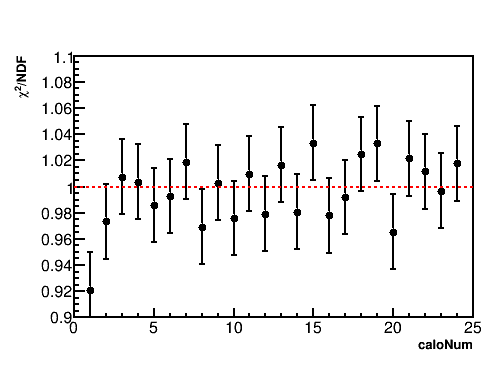
\includegraphics[width=\textwidth]{FullRatioFit_Chi2NDF_Vs_Calo_Canv_60h}
        \caption{}
    \end{subfigure}% %you need this % here to add spacing between subfigures
    \begin{subfigure}[]{0.45\textwidth}
        \centering
        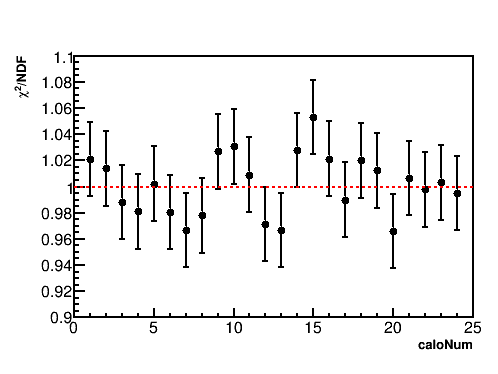
\includegraphics[width=\textwidth]{FullRatioFit_Chi2NDF_Vs_Calo_Canv_HighKick}
        \caption{}
    \end{subfigure}

    \begin{subfigure}[]{0.45\textwidth}
        \centering
        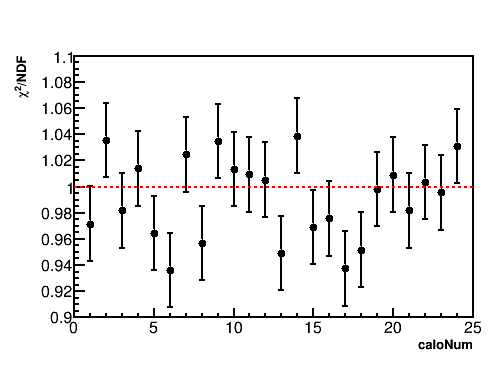
\includegraphics[width=\textwidth]{FullRatioFit_Chi2NDF_Vs_Calo_Canv_9d}
        \caption{}
    \end{subfigure}% %you need this % here to add spacing between subfigures
    \begin{subfigure}[]{0.45\textwidth}
        \centering
        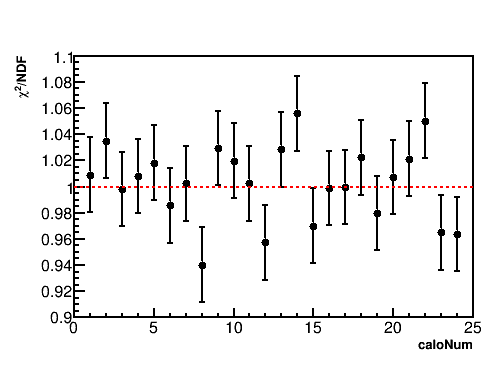
\includegraphics[width=\textwidth]{FullRatioFit_Chi2NDF_Vs_Calo_Canv_Endgame}
        \caption{}
    \end{subfigure}
\caption[]{chi2s calo fits Data from some dataset.}
\label{fig:}
\end{figure}


\begin{figure}[]
\centering
    \begin{subfigure}[]{0.45\textwidth}
        \centering
        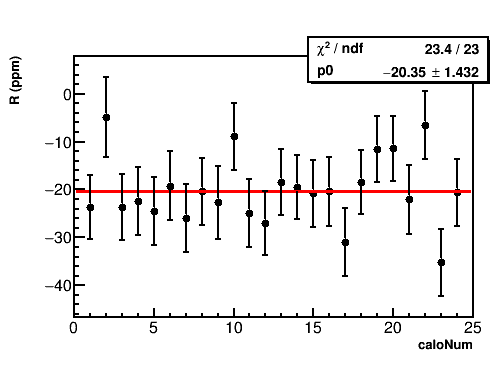
\includegraphics[width=\textwidth]{FullRatioFit_R_Vs_Calo_Canv_60h}
        \caption{}
    \end{subfigure}% %you need this % here to add spacing between subfigures
    \begin{subfigure}[]{0.45\textwidth}
        \centering
        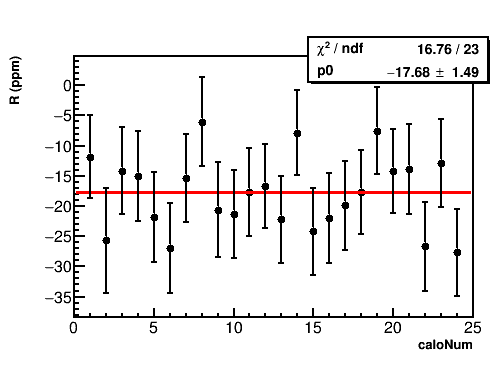
\includegraphics[width=\textwidth]{FullRatioFit_R_Vs_Calo_Canv_HighKick}
        \caption{}
    \end{subfigure}

    \begin{subfigure}[]{0.45\textwidth}
        \centering
        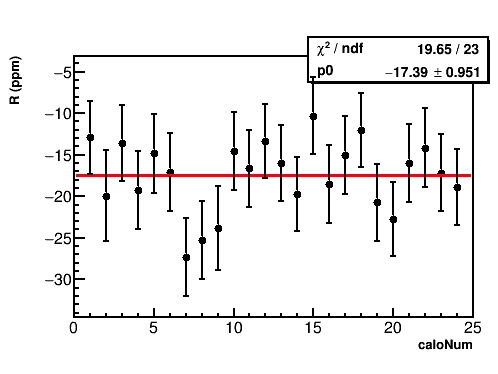
\includegraphics[width=\textwidth]{FullRatioFit_R_Vs_Calo_Canv_9d}
        \caption{}
    \end{subfigure}% %you need this % here to add spacing between subfigures
    \begin{subfigure}[]{0.45\textwidth}
        \centering
        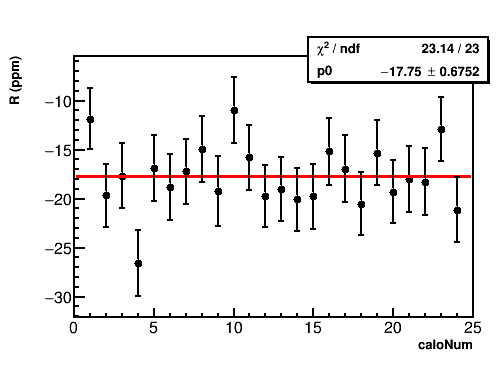
\includegraphics[width=\textwidth]{FullRatioFit_R_Vs_Calo_Canv_Endgame}
        \caption{}
    \end{subfigure}
\caption[]{Rs calo fits Data from some dataset.}
\label{fig:}
\end{figure}


\begin{figure}[]
\centering
    \begin{subfigure}[]{0.45\textwidth}
        \centering
        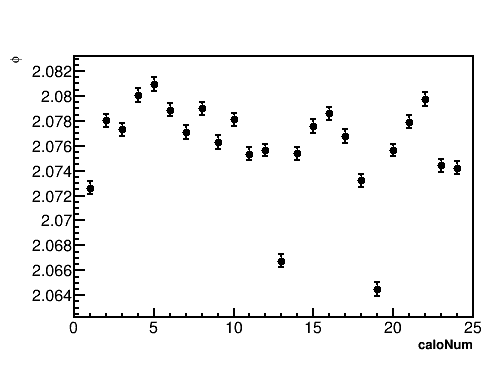
\includegraphics[width=\textwidth]{FullRatioFit_phi_Vs_Calo_Canv_Endgame}
        \caption{}
    \end{subfigure}% %you need this % here to add spacing between subfigures
    \begin{subfigure}[]{0.45\textwidth}
        \centering
        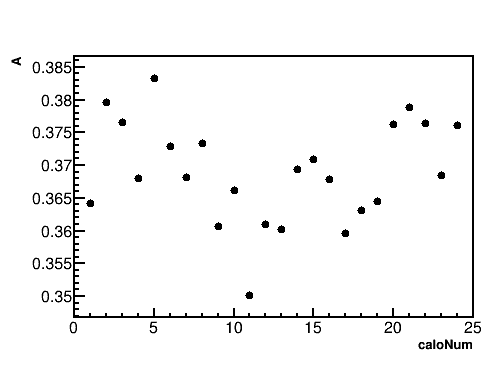
\includegraphics[width=\textwidth]{FullRatioFit_A_Vs_Calo_Canv_Endgame}
        \caption{}
    \end{subfigure}

    \begin{subfigure}[]{0.45\textwidth}
        \centering
        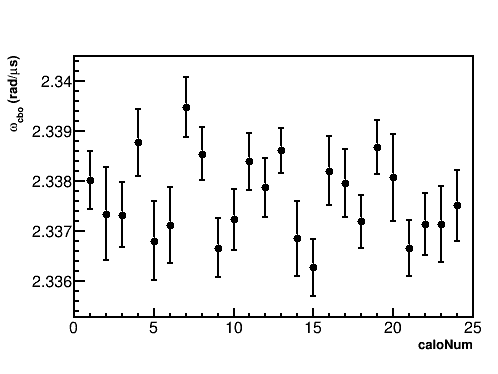
\includegraphics[width=\textwidth]{FullRatioFit_omega_cbo_Vs_Calo_Canv_Endgame}
        \caption{}
    \end{subfigure}% %you need this % here to add spacing between subfigures
    \begin{subfigure}[]{0.45\textwidth}
        \centering
        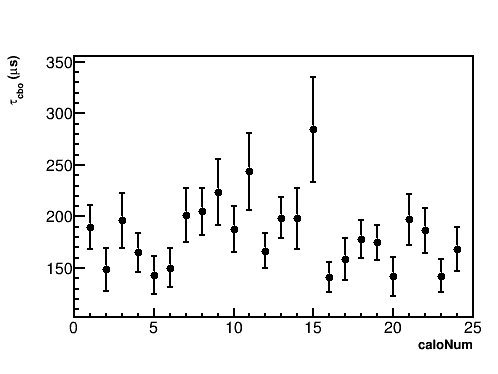
\includegraphics[width=\textwidth]{FullRatioFit_tau_cbo_Vs_Calo_Canv_Endgame}
        \caption{}
    \end{subfigure}

    \begin{subfigure}[]{0.45\textwidth}
        \centering
        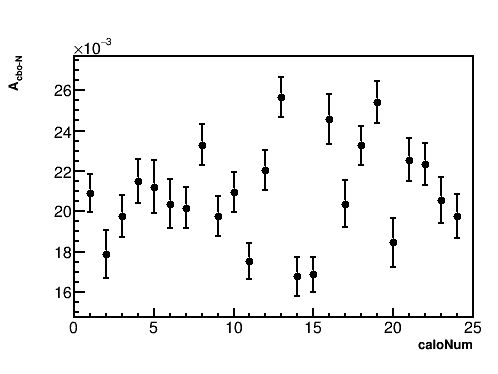
\includegraphics[width=\textwidth]{FullRatioFit_A_cbo-N_Vs_Calo_Canv_Endgame}
        \caption{}
    \end{subfigure}% %you need this % here to add spacing between subfigures
    \begin{subfigure}[]{0.45\textwidth}
        \centering
        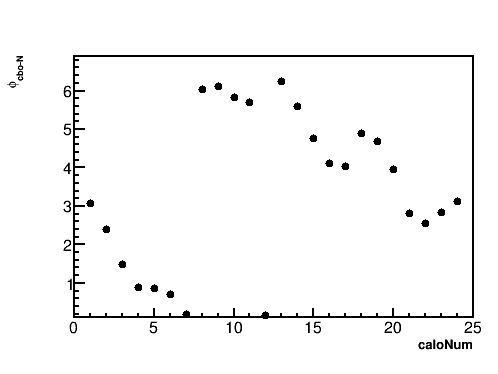
\includegraphics[width=\textwidth]{FullRatioFit_phi_cbo-N_Vs_Calo_Canv_Endgame}
        \caption{}
    \end{subfigure}
\caption[]{Endgame calo fits Data from some dataset.}
\label{fig:}
\end{figure}


\begin{figure}[]
\centering
    \begin{subfigure}[]{0.45\textwidth}
        \centering
        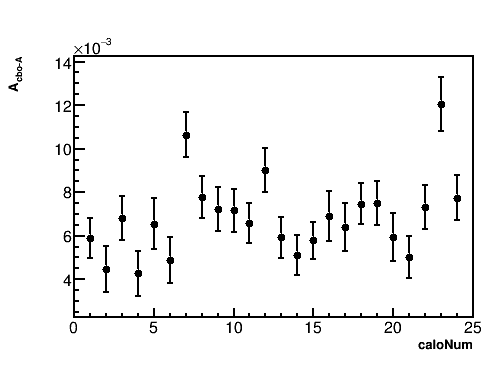
\includegraphics[width=\textwidth]{FullRatioFit_A_cbo-A_Vs_Calo_Canv_Endgame}
        \caption{}
    \end{subfigure}% %you need this % here to add spacing between subfigures
    \begin{subfigure}[]{0.45\textwidth}
        \centering
        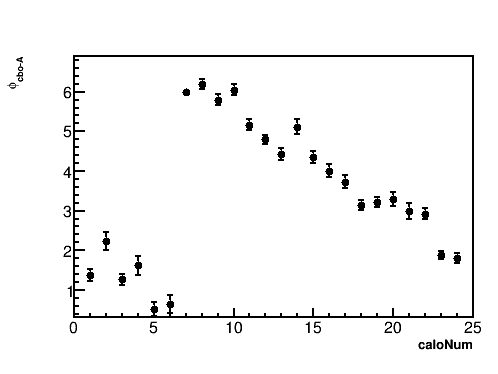
\includegraphics[width=\textwidth]{FullRatioFit_phi_cbo-A_Vs_Calo_Canv_Endgame}
        \caption{}
    \end{subfigure}

    \begin{subfigure}[]{0.45\textwidth}
        \centering
        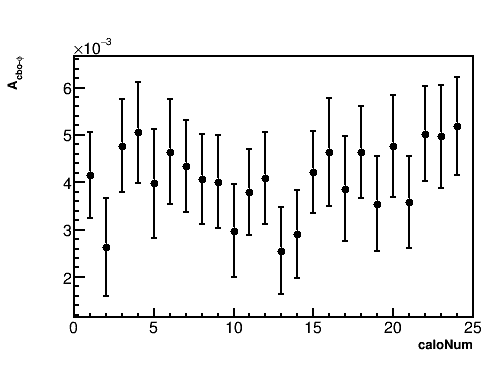
\includegraphics[width=\textwidth]{FullRatioFit_A_cbo-phi_Vs_Calo_Canv_Endgame}
        \caption{}
    \end{subfigure}% %you need this % here to add spacing between subfigures
    \begin{subfigure}[]{0.45\textwidth}
        \centering
        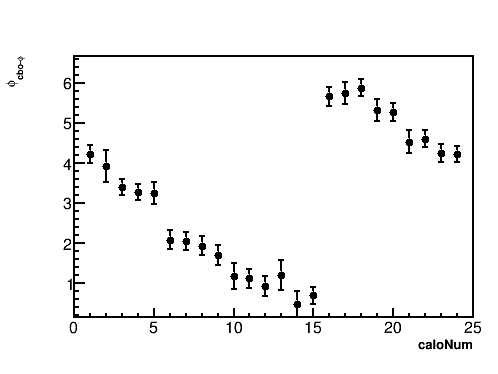
\includegraphics[width=\textwidth]{FullRatioFit_phi_cbo-phi_Vs_Calo_Canv_Endgame}
        \caption{}
    \end{subfigure}

    \begin{subfigure}[]{0.45\textwidth}
        \centering
        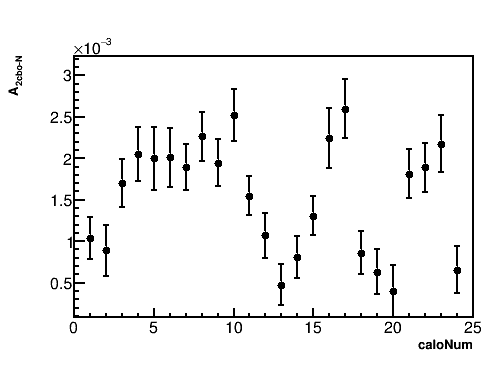
\includegraphics[width=\textwidth]{FullRatioFit_A_2cbo-N_Vs_Calo_Canv_Endgame}
        \caption{}
    \end{subfigure}% %you need this % here to add spacing between subfigures
    \begin{subfigure}[]{0.45\textwidth}
        \centering
        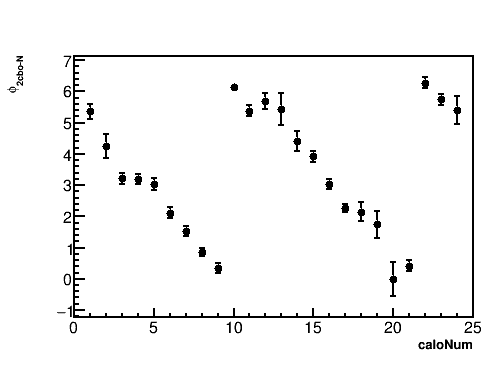
\includegraphics[width=\textwidth]{FullRatioFit_phi_2cbo-N_Vs_Calo_Canv_Endgame}
        \caption{}
    \end{subfigure}
\caption[]{Endgame calo fits Data from some dataset.}
\label{fig:}
\end{figure}



-put here per calo fits of endgame dataset parameters besides chi2 and R


\subsection{Fit start scans}

-include here the Kawall band equation as well as the full form

\begin{figure}[]
\centering
    \begin{subfigure}[]{0.45\textwidth}
        \centering
        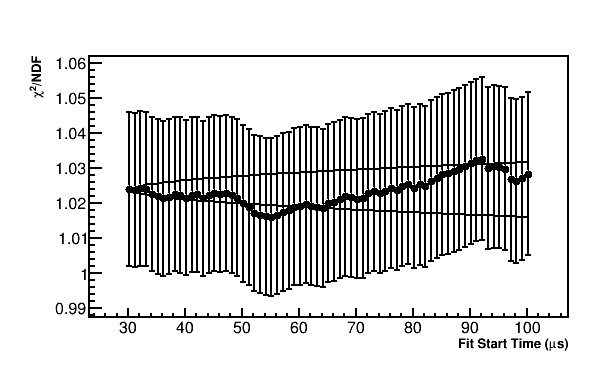
\includegraphics[width=\textwidth]{FullRatio_Chi2NDF_Vs_FS_canv_60h}
        \caption{}
    \end{subfigure}% %you need this % here to add spacing between subfigures
    \begin{subfigure}[]{0.45\textwidth}
        \centering
        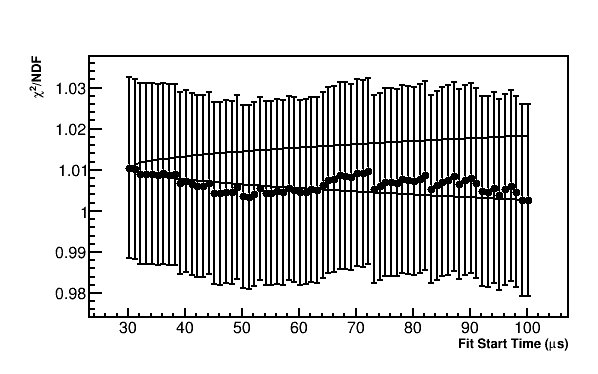
\includegraphics[width=\textwidth]{FullRatio_Chi2NDF_Vs_FS_canv_HighKick}
        \caption{}
    \end{subfigure}

    \begin{subfigure}[]{0.45\textwidth}
        \centering
        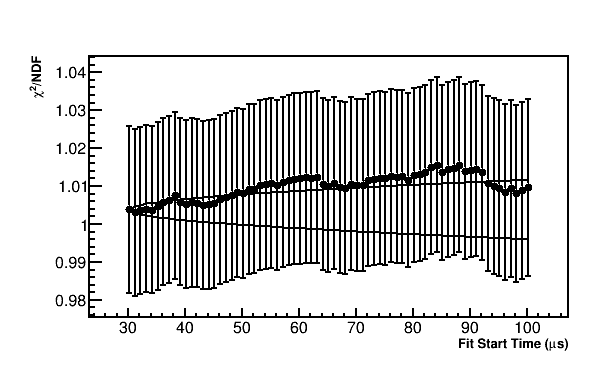
\includegraphics[width=\textwidth]{FullRatio_Chi2NDF_Vs_FS_canv_9d}
        \caption{}
    \end{subfigure}% %you need this % here to add spacing between subfigures
    \begin{subfigure}[]{0.45\textwidth}
        \centering
        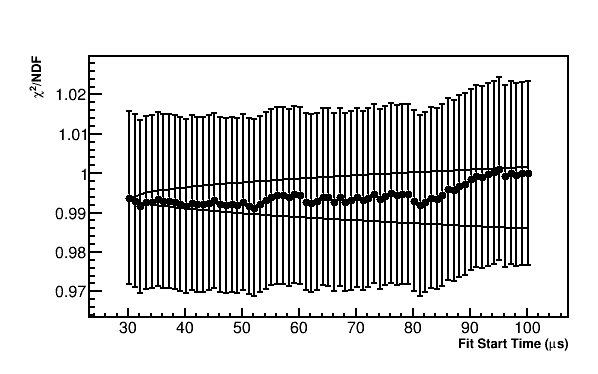
\includegraphics[width=\textwidth]{FullRatio_Chi2NDF_Vs_FS_canv_Endgame}
        \caption{}
    \end{subfigure}
\caption[]{chi2s fit start Data from some dataset.}
\label{fig:}
\end{figure}

\begin{figure}[]
\centering
    \begin{subfigure}[]{0.45\textwidth}
        \centering
        \includegraphics[width=\textwidth]{FullRatio_R_FS_canv_60h}
        \caption{}
    \end{subfigure}% %you need this % here to add spacing between subfigures
    \begin{subfigure}[]{0.45\textwidth}
        \centering
        \includegraphics[width=\textwidth]{FullRatio_R_FS_canv_HighKick}
        \caption{}
    \end{subfigure}

    \begin{subfigure}[]{0.45\textwidth}
        \centering
        \includegraphics[width=\textwidth]{FullRatio_R_FS_canv_9d}
        \caption{}
    \end{subfigure}% %you need this % here to add spacing between subfigures
    \begin{subfigure}[]{0.45\textwidth}
        \centering
        \includegraphics[width=\textwidth]{FullRatio_R_FS_canv_Endgame}
        \caption{}
    \end{subfigure}
\caption[]{R fit starts Data from some dataset.}
\label{fig:}
\end{figure}


\begin{figure}[]
\centering
    \begin{subfigure}[]{0.45\textwidth}
        \centering
        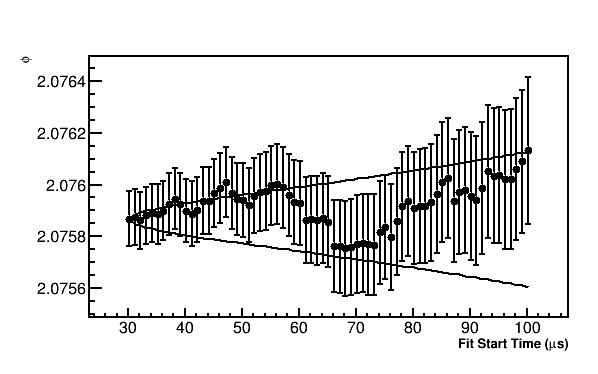
\includegraphics[width=\textwidth]{FullRatio_phi_FS_Canv_Endgame}
        \caption{}
    \end{subfigure}% %you need this % here to add spacing between subfigures
    \begin{subfigure}[]{0.45\textwidth}
        \centering
        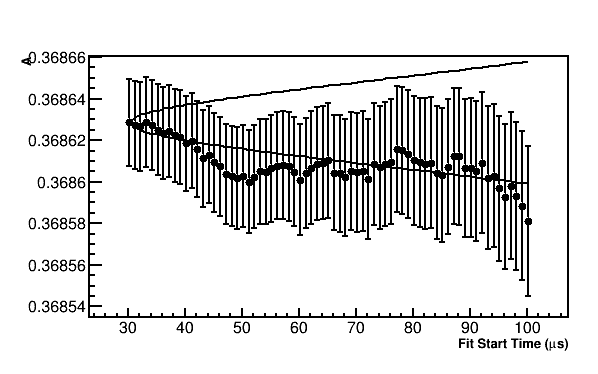
\includegraphics[width=\textwidth]{FullRatio_A_FS_Canv_Endgame}
        \caption{}
    \end{subfigure}

    \begin{subfigure}[]{0.45\textwidth}
        \centering
        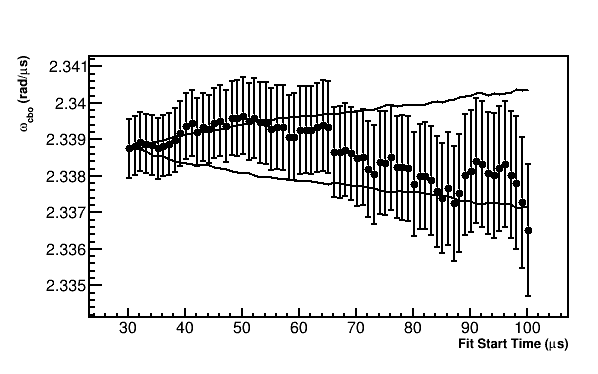
\includegraphics[width=\textwidth]{FullRatio_omega_cbo_FS_Canv_Endgame}
        \caption{}
    \end{subfigure}% %you need this % here to add spacing between subfigures
    \begin{subfigure}[]{0.45\textwidth}
        \centering
        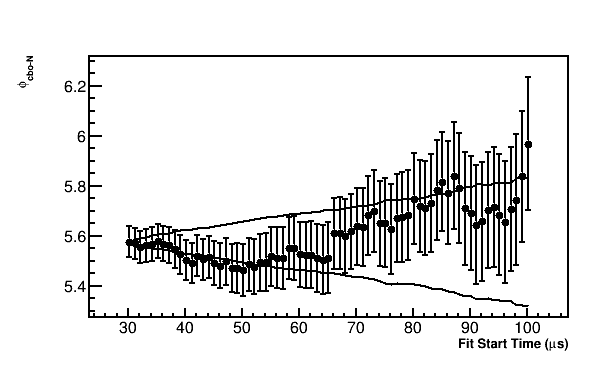
\includegraphics[width=\textwidth]{FullRatio_phi_cbo-N_FS_Canv_Endgame}
        \caption{}
    \end{subfigure}

    \begin{subfigure}[]{0.45\textwidth}
        \centering
        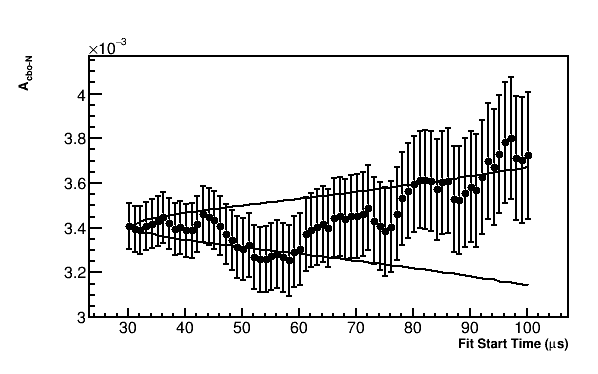
\includegraphics[width=\textwidth]{FullRatio_A_cbo-N_FS_Canv_Endgame}
        \caption{}
    \end{subfigure}% %you need this % here to add spacing between subfigures
    \begin{subfigure}[]{0.45\textwidth}
        \centering
        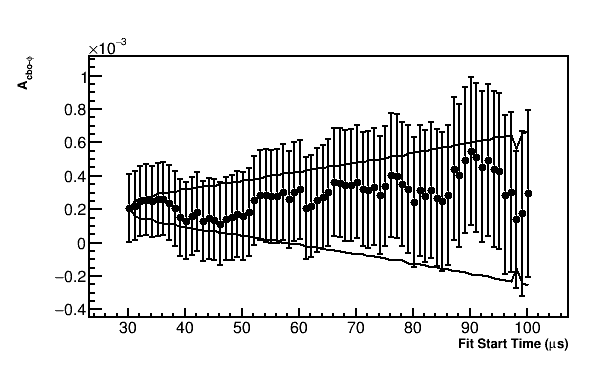
\includegraphics[width=\textwidth]{FullRatio_A_cbo-phi_FS_Canv_Endgame}
        \caption{}
    \end{subfigure}
\caption[]{other parameter fit starts endgame - missing plots are those for fixed parameters Data from some dataset.}
\label{fig:}
\end{figure}


\subsection{Fit end scans}


\begin{figure}[]
\centering
    \begin{subfigure}[]{0.45\textwidth}
        \centering
        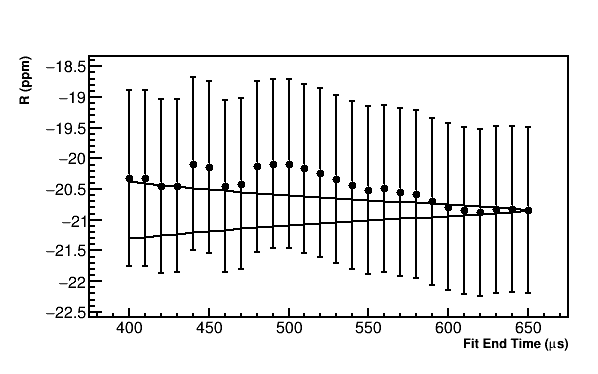
\includegraphics[width=\textwidth]{FullRatio_R_FE_Canv_60h}
        \caption{}
    \end{subfigure}% %you need this % here to add spacing between subfigures
    \begin{subfigure}[]{0.45\textwidth}
        \centering
        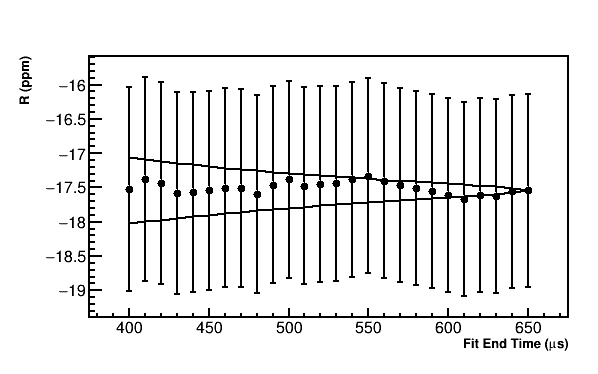
\includegraphics[width=\textwidth]{FullRatio_R_FE_Canv_HighKick}
        \caption{}
    \end{subfigure}

    \begin{subfigure}[]{0.45\textwidth}
        \centering
        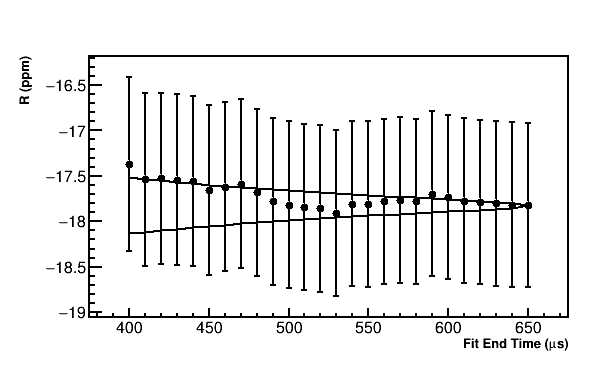
\includegraphics[width=\textwidth]{FullRatio_R_FE_Canv_9d}
        \caption{}
    \end{subfigure}% %you need this % here to add spacing between subfigures
    \begin{subfigure}[]{0.45\textwidth}
        \centering
        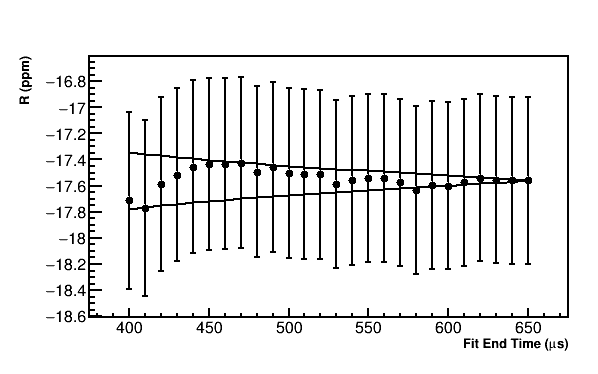
\includegraphics[width=\textwidth]{FullRatio_R_FE_Canv_Endgame}
        \caption{}
    \end{subfigure}
\caption[]{R fit ends Data from some dataset.}
\label{fig:}
\end{figure}


\subsection{Energy threshold scan fits}

-should include here plots of A and N as well as R - though maybe I should move them up to the histogram construction side of things

\begin{figure}[]
\centering
    \begin{subfigure}[]{0.45\textwidth}
        \centering
        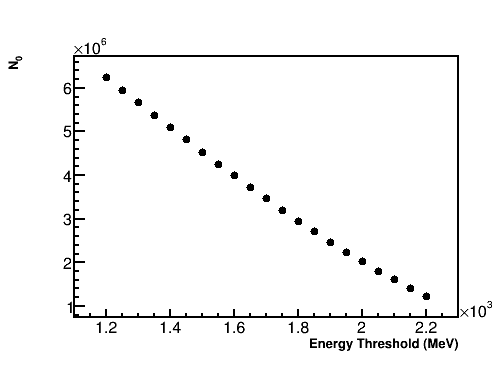
\includegraphics[width=\textwidth]{FiveParameter_N_0_Vs_ETh_60h}
        \caption{}
    \end{subfigure}% %you need this % here to add spacing between subfigures
    \begin{subfigure}[]{0.45\textwidth}
        \centering
        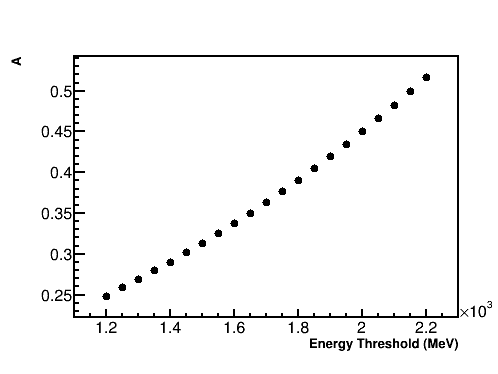
\includegraphics[width=\textwidth]{FiveParameter_A_Vs_ETh_60h}
        \caption{}
    \end{subfigure}
\caption[]{60h five parameter fit N and A Data from some dataset.}
\label{fig:}
\end{figure}



\begin{figure}[]
\centering
    \begin{subfigure}[]{0.45\textwidth}
        \centering
        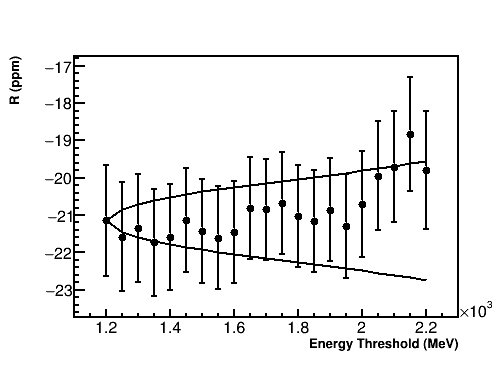
\includegraphics[width=\textwidth]{FullRatio_R_Vs_ETh_60h}
        \caption{}
    \end{subfigure}% %you need this % here to add spacing between subfigures
    \begin{subfigure}[]{0.45\textwidth}
        \centering
        \includegraphics[width=\textwidth]{FullRatio_R_Vs_ETh_HighKick}
        \caption{}
    \end{subfigure}

    \begin{subfigure}[]{0.45\textwidth}
        \centering
        \includegraphics[width=\textwidth]{FullRatio_R_Vs_ETh_9d}
        \caption{}
    \end{subfigure}% %you need this % here to add spacing between subfigures
    \begin{subfigure}[]{0.45\textwidth}
        \centering
        \includegraphics[width=\textwidth]{FullRatio_R_Vs_ETh_Endgame}
        \caption{}
    \end{subfigure}
\caption[]{R energy threshold scans Data from some dataset.}
\label{fig:}
\end{figure}





\subsection{Fits to bunch number}

- this should maybe go up by fit results section


\begin{figure}[]
\centering
    \begin{subfigure}[]{0.45\textwidth}
        \centering
        \includegraphics[width=\textwidth]{FullRatio_R_Vs_BunchNum_Canv_60h}
        \caption{}
    \end{subfigure}% %you need this % here to add spacing between subfigures
    \begin{subfigure}[]{0.45\textwidth}
        \centering
        \includegraphics[width=\textwidth]{FullRatio_R_Vs_BunchNum_Canv_HighKick}
        \caption{}
    \end{subfigure}

    \begin{subfigure}[]{0.45\textwidth}
        \centering
        \includegraphics[width=\textwidth]{FullRatio_R_Vs_BunchNum_Canv_9d}
        \caption{}
    \end{subfigure}% %you need this % here to add spacing between subfigures
    \begin{subfigure}[]{0.45\textwidth}
        \centering
        \includegraphics[width=\textwidth]{FullRatio_R_Vs_BunchNum_Canv_Endgame}
        \caption{}
    \end{subfigure}
\caption[]{R bunch nums Data from some dataset.}
\label{fig:}
\end{figure}



\subsection{Fits to many random seeds}

-make a table of results with RMS and errors on the mean
-point out how HighKick, 9d, and Endgame are all consistent, and remind that 60h has a different blinding



\begin{figure}[]
\centering
    \begin{subfigure}[]{0.45\textwidth}
        \centering
        \includegraphics[width=\textwidth]{FullRatio_Chi2NDF_Vs_Iter_Canv_hist_60h}
        \caption{}
    \end{subfigure}% %you need this % here to add spacing between subfigures
    \begin{subfigure}[]{0.45\textwidth}
        \centering
        \includegraphics[width=\textwidth]{FullRatio_Chi2NDF_Vs_Iter_Canv_hist_HighKick}
        \caption{}
    \end{subfigure}

    \begin{subfigure}[]{0.45\textwidth}
        \centering
        \includegraphics[width=\textwidth]{FullRatio_Chi2NDF_Vs_Iter_Canv_hist_9d}
        \caption{}
    \end{subfigure}% %you need this % here to add spacing between subfigures
    \begin{subfigure}[]{0.45\textwidth}
        \centering
        \includegraphics[width=\textwidth]{FullRatio_Chi2NDF_Vs_Iter_Canv_hist_Endgame}
        \caption{}
    \end{subfigure}
\caption[]{chi2 fits to many seeds Data from some dataset.}
\label{fig:}
\end{figure}


\begin{figure}[]
\centering
    \begin{subfigure}[]{0.45\textwidth}
        \centering
        \includegraphics[width=\textwidth]{FullRatio_R_Vs_Iter_Canv_hist_60h}
        \caption{}
    \end{subfigure}% %you need this % here to add spacing between subfigures
    \begin{subfigure}[]{0.45\textwidth}
        \centering
        \includegraphics[width=\textwidth]{FullRatio_R_Vs_Iter_Canv_hist_HighKick}
        \caption{}
    \end{subfigure}

    \begin{subfigure}[]{0.45\textwidth}
        \centering
        \includegraphics[width=\textwidth]{FullRatio_R_Vs_Iter_Canv_hist_9d}
        \caption{}
    \end{subfigure}% %you need this % here to add spacing between subfigures
    \begin{subfigure}[]{0.45\textwidth}
        \centering
        \includegraphics[width=\textwidth]{FullRatio_R_Vs_Iter_Canv_hist_Endgame}
        \caption{}
    \end{subfigure}
\caption[]{R fits to many seeds Data from some dataset.}
\label{fig:}
\end{figure}


\clearpage % remove this once things are sorted






% \begin{figure}[]
%     \centering
%     \includegraphics[width=.8\textwidth]{}
%     \caption[]{Data from some dataset.}
%     \label{fig:}
% \end{figure}

% \begin{figure}[]
% \centering
%     \begin{subfigure}[]{0.8\textwidth}
%         \centering
%         \includegraphics[width=\textwidth]{}
%         \caption{}
%     \end{subfigure}% %you need this % here to add spacing between subfigures
%     \vspace{1cm}
%     \begin{subfigure}[]{0.8\textwidth}
%         \centering
%         \includegraphics[width=\textwidth]{}
%         \caption{}
%     \end{subfigure}
% \caption[]{Data from some dataset.}
% \label{fig:}
% \end{figure}

% \begin{figure}[]
% \centering
%     \begin{subfigure}[]{0.45\textwidth}
%         \centering
%         \includegraphics[width=\textwidth]{}
%         \caption{}
%     \end{subfigure}% %you need this % here to add spacing between subfigures
%     \begin{subfigure}[]{0.45\textwidth}
%         \centering
%         \includegraphics[width=\textwidth]{}
%         \caption{}
%     \end{subfigure}

%     \begin{subfigure}[]{0.45\textwidth}
%         \centering
%         \includegraphics[width=\textwidth]{}
%         \caption{}
%     \end{subfigure}% %you need this % here to add spacing between subfigures
%     \begin{subfigure}[]{0.45\textwidth}
%         \centering
%         \includegraphics[width=\textwidth]{}
%         \caption{}
%     \end{subfigure}
% \caption[]{Data from some dataset.}
% \label{fig:}
% \end{figure}
